\section{Multi-Party Computation based Process Mining}
\label{sec:approach}
This section introduce our techniques for process mining based on 
secure multi-party computation. To this end, in \autoref{sec:model}, we first 
clarify our model for cross-organizational process mining including the 
required input data and the obtained analysis results. We then introduce our 
architecture for realizing the respective analysis using secure multi-party 
computation in \autoref{sec:core_approach}. In 
\autoref{sec:div_and_conq}, we focus on techniques for vectorization and 
parallelization to improve the efficiency of our approach.

\subsection{Model for Cross-organizational Process Mining}
\label{sec:model}

We consider a model in which an event log $L=\{t_1,\ldots,t_n\}$ is defined as 
a set of traces, each capturing the single execution of a business 
process. We define a trace $t$ as a finite sequence of events $t=\langle 
e_1,\ldots,e_m \rangle$. An event $e$ is defined as $e=(i,a,ts)$. It represents 
a single execution of an activity $a$ at time $ts$, where $i$ is 
a unique event identifier, i.e., $i = i'$ implies that $(i,a,ts) = 
(i',a',ts')$. We assume that events in a trace are ordered by their timestamp. 

However, for a cross-organizational business process, an event log that records 
the process execution from start to end is commonly not available. Rather, 
different parties record sub-logs that contain sub-traces, built of events that 
denote activity executions at the respective party. To keep the notation 
concise, we consider a setting in which two parties, $I_a$ and $I_b$, execute a 
cross-organizational process, e.g., the airport and the airline in our 
motivating example. Then, each of the two parties records an event log, denoted 
by $L_a$ and $L_b$. A trace $t=\langle 
e_1,\ldots,e_m \rangle\in L$ of the cross-organizational process is 
materialized as two sub-traces, $t_a \in L_a$ and $t_b \in L_b$, each being 
defined as the order-preserving projection of trace $t$ on the events that 
denote activity executions at the respective parties $I_a$ and $I_b$. We assume 
that each activity can only be executed by one of the parties, so that the 
projection of the log into sub-logs is defined unambiguously. 

For the above setting, we consider the scenario that the parties $I_a$ and 
$I_b$ want to answer some analysis queries $Q$ over the cross-organizational 
event log $L$, yet \emph{without} sharing their logs $L_a$ and $L_b$ with each 
other. 
More specifically, we focus on analysis queries that can be answered on a 
time-annotated directly-follows-graph (DFG) of the cross-organizational 
process. \todo{@Stephan, could you clarify that DFG would be kept secret in sharemind and we reveal only the answers for the queries?} In essence, the DFG captures the frequencies with which the executions 
of two activities have been observed to directly follow upon each other in a 
trace. Moreover, we consider temporal annotations of the directly-follows 
dependencies in terms of time between the respective activity executions. A 
time-annotated DFG thereby enables conclusions on the main paths of process 
execution, rarely executed paths, as well as the location of major delays in 
processing.

Formally, the time-annotated DFG is captured by an $|A| \times |A|$ matrix, 
where $A$ is the set of all possible activities of the process. Each cell 
contains a tuple $(c,\Delta)$. The counter $c$ represents the frequency with 
which a directly-follows dependency has been observed in $L$, i.e., for the 
cell $(a_1,a_2)$ it is the number of times that two events $e_1=(i_1,a_1,ts_1)$ 
and $e_2=(i_2,a_2,ts_2)$ follow each other directly in some trace of $L$. 
Furthermore, 
$\Delta$ is the total sum of the time that passed by between all occurrences of 
the respective events, i.e., $ts_2 - ts_1$ for the above events. 

In cross-organizational process mining, the aforementioned time-annotated DFG 
cannot be computed directly, as this would require the two parties to share and 
integrate their sub-logs. 


%To enable process mining in a cross-organizational setting we assume that the 
%queries the organizations want to execute can be answered by subset of the 
%elements of the annotated \emph{directly-follows-graph} (DFG) of the 
%cross-organizational process.
%Additionally, we consider that we have two input parties $I_a$ and $I_b$, such 
%as an airport and an airline in our motivational example. 
%These input parties 
%have access to there respective event logs $L_a$ and $L_b$, with $L_a \cap L_b 
%=\emptyset$. While the whole business process is represented by the event log 
%$L = L_a \cup L_b$. We define a log $L$ as a set of traces, 
%$L=\{t_1,...,t_n\}$. Each trace $t$ captures the single execution of a 
%business 
%process. We define a trace $t$ as a finite sequence of events $t=\langle 
%e_1,...,e_m \rangle$. Where is event $e$ is defined as $e=(i,a,ts) $ and 
%represents the single execution of an activity $a$ at time $ts$. With $i$ 
%being 
%the event identifier such as $i = i'$ implies that $(i,a,ts) = (i',a',ts')$. 
%For our cross-organizational setting we assume that a trace $t \in L$ 
%corresponds to subtraces $t_a \in L_a$ and $t_b \in L_b$, such as $t = t_a 
%\cup 
%t_b$. As an additional assumption we assume that an activity $a$ that is 
%executed by one party, e.g.,$I_a$, can not be executed by the other party, 
%e.g. 
%$I_b$.
%
%We assume that the input parties $I_a$ and $I_b$ want to calculate some 
%queries 
%$Q$ over the cross-organizational event log $L$ without sharing their 
%respective logs $L_a$ and $L_b$ with each other. However, to answer the 
%queries 
%in $Q$ they must generate the DFG over their combined event log $L$. The 
%annotated DFG is a matrix based on $ A \times A$, where $A$ is the universe of 
%all possible activities in $L$. Each cell of the DFG matrix contains a tuple 
%$(c,\Delta)$. The counter $c$ represents the times a 
%directly-follows-relations 
%appeared, e.g. an event $e_2$ of activity $a_2$ was executed after an event 
%$e_1$ of activity $a_1$ appeared in trace $t_1$, and the total sum of time 
%$\Delta$ that passed by between all occurrences of that 
%directly-follow-relations, so for our trace $t_1$ the time passed would be 
%$\Delta_1 = ts_2 - ts_1$ with $ ts_1 \in e_1,  ts_2 \in e_2 $.

\subsection{MPC Architecture for Process Mining}
\label{sec:core_approach}

In order to enable inter-organizational process mining based on a 
time-annotated DFG \emph{without} requiring parties to sharing their event logs 
with each other, we propose an architecture for secure multi-party computation 
(MPC). As outlined in \autoref{fig:overview}, we rely on a platform for MPC 
that takes the event logs of the participating parties, i.e., $L_a$ and $L_b$, 
as encrypted input. In the MPC platform, the respective data is then prepared 
in several steps in order to answer analysis queries over the time-annotated 
DFG. 

%Since we believe we sharing the complete DFG would reveal to much confidential 
%information in most scenarios, we would only release a subset of the cells of 
%the DFG based on some queries $Q$. 

\begin{figure}[!htb]
	\centering
	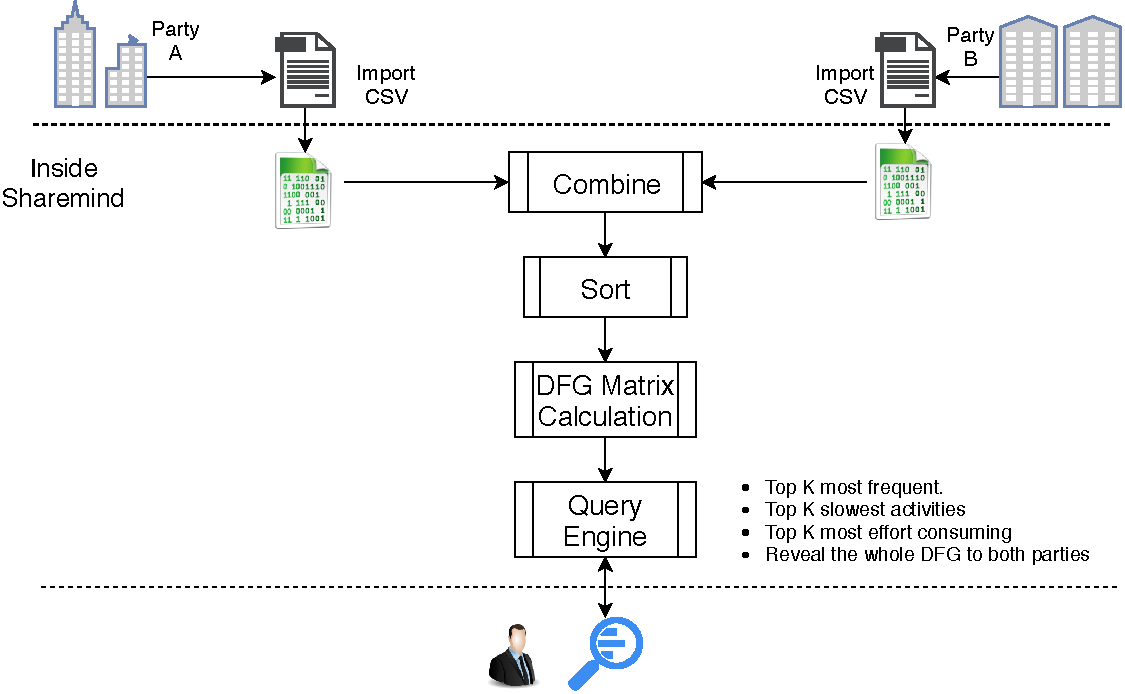
\includegraphics[width=.95\columnwidth]{figures/mpc_algorithm}
	\caption{Number of variants retained for $k$-anonymity.}
	\label{fig:overview}
\end{figure}

\noindent
We summarize the functionality realized in the MPC platform as 
follows:
\begin{compactitem}
\item[\emph{Combination}] While the input parties upload their respective event logs $L_a$ and $L_b$ to the MPC platform, these get encrypted and distributed to the computing parties. So it is ensured, that nobody can access the secret data. After the logs upload we append one of the logs to the other so that the unsorted log $L$ is created.
\item[\emph{Sorting}] To ensure an efficient calculation of the annotated DFG $G$ we sort the merged log $L$, such that all event $e \in t$ of a trace $t \in L$ are group together and ordered by their respective execution time $ts$. For this purpose we rely on the network sorting algorithm\cite{bogdanov2014practical}, that ensures efficient sorting without revealing secret information.
\item[\emph{Matrix calculation}] After sorting $L$ we can construct the DFG $G$ inside the MPC platform, while keeping the DFG $G$ secret and not revealing any information.
\item[\emph{Query answering}] A query $Q$ requests a subset $S$ of the annotated DFG $G$. The MPC platform generates $S$ based on the query $Q$, e.g., the top-5 most common activities, and only reveals this subset $S$ to the output parties. By publishing only the subsets $S$ to pre-defined output parties we limit the information an output party can learn about the process. 
\end{compactitem}

%It consists of several major steps, starting with merging the secret 
%logs $L_a$ and $L_b$ by appending them to each other and then sorting them, 
%such that all event $e \in t$ of a trace $t \in L$ are group together and 
%ordered by their respective execution time $ts$. To ensure an efficient 
%execution of such sorting we rely on the network sorting 
%algorithm\cite{bogdanov2014practical}. Following the sorting we construct the 
%DFG based on the algorithm~\ref{alg:merge}.

%After construction the combined DFG $G$ we can apply the queries $Q$ and retrieve the respective subsets $S$ of $G$. Each subset $s \in S$ represents the answer to one query $q \in Q$. By publishing only the subsets $S$ to pre-defined output parties we limit the information an output party can learn about the process. 

%\begin{algorithm}[!htb]
%	\caption{Calculating the combined, annotated DFG($L$)}
%	\label{alg:merge}
%	\begin{flushleft}
%		\textbf{INPUT:} The sorted combined event log $L$\\
%		\textbf{OUTPUT:} DFG $G$, Waiting time matrix $W$
%		\vspace{-.4em}
%	\end{flushleft}
%	\begin{algorithmic}[1]
%		\State Initialize $G$,$W$
%		\ForAll{$t \in \mathit{L}$} \label{line:all_cases}
%			\State currentEvent $\gets$ startEvent
%			\Repeat
%				\State $G_a$ = currentEvent * nextEvent($t$).reshape()
%				\State $W$ = $G_a$ *  (nextEvent($t$).timestamp - currentEvent.timestamp)
%			\Until nextEvent($t$) $ = \emptyset$ 
%		\EndFor
%		\State \Return $G$, $W$
%	\end{algorithmic}
%\end{algorithm}

%Algorithm~\ref{alg:merge} shows the respective algorithm. Our approach keeps both event logs separated and only calculates the combined DFG. Alternatively, it would be possible to merge both logs $L_a$ and $L_a$ into one log $L$ and then calculate the DFG over $L$. However, this would require sorting the merged  log $L$ based on the time an event happened, to enable calculating the DFG. But sorting has the complexity of $\mathcal{O}(n \log n)$ and our algorithm has the complexity of $\mathcal{O}(n)$, with $n$ being the number of events in $L = L_a \cup L_b$. Therefore, Algorithm~\ref{alg:merge} ensures faster performance compared to a  simple merge of $L_a$ and $L_b$.


\subsection{Scalability Considerations}
\label{sec:div_and_conq}

Cross-organizational process mining using the above general architecture might 
suffer from scalability issues. The reason being the use of multi-party 
computation to realise the functionality to combine and sort the event logs and 
to calculate the annotated DFG, which is inherently distributed and applied to 
homomorphic encrypted data. Hence, even 
for functions that have a generally low run-time complexity ($\mathcal{O}(n)$ 
for the combination, $\mathcal{O}(n\log(n))$ for the sorting, 
$\mathcal{O}(n^2)$ for 
the calculation of the annotated DFG), there is a non-negligible overhead 
induced by MPC. For instance, a naive realisation of the Quicksort algorithm to 
sort the events of the combined log would require $\mathcal{O}(n\log(n))$ 
rounds of communication between the distributed nodes and 
$\mathcal{O}(n\log(n))$ value comparisons per round~\cite{Hamada12}. Against 
this background, we consider two angles to improve the efficiency of 
the analysis, namely vectorization and parallelization. 

\paragraph{Vectorization.} Contemporary MPC platforms provide efficient 
implementations of basic functions to process distributed, encrypted data. 
For instance, Sharemind supports bitwise secret sharing that represents a data 
value as a bitwise combination of vectors that are distributed among the nodes. 
Based thereon, the platform offers efficient implementations of vector-based 
functions, such as those for matrix 
multiplication~\cite{kerik2016optimizing,laud2017privacy}. For instance, the 
multiplication of two bit vectors can be realized in one round that requires 
$\mathcal{O}(6k)$ interactions between nodes, where $k$ is the number of bits 
required to encode the value. 

To leverage the efficient implementation of such basic functions, we employ 
vectorization and represent events as a bit vector over the set $A$ of all 
possible activities of the process. To mask the actual number of possible 
activities, the set over which the vector is defined may include padding, i.e., 
some additional placeholders. Following this representation, an event 
corresponds to a binary vector in which at most one bit is set to one. Then, 
counting the number of directly-follows dependencies in the computation of the 
annotated DFG can be traced back to vector multiplication. 


\todo{Matthias, rework the following}
\paragraph{Parallelization.}
An additional approach to improve the runtime performance common for 
secure-multi party computation is the usage of parallelization. To ensure 
efficient parallelization it is important to divide the data from the input 
parties such that all data chunks can be used independent from each other. In 
our scenario this can be done by bundling chunks of cases and distributing them 
to several machine.  For each chunk a DFG can be generated. The different DFGs 
can then be united to one DFG that represents the entire business process. 

However, such an approach comes with the question of determining the size of the chunks. We consider that a chunk has size $m$ representing the number of cases that are at least part of that chunk. In a multi-party computation setting the result of the processing of each chunk would not be protected. Therefore, proceeding only a small number of cases in one chunk might reveal a lot of information about the cases inside the chunk and is critical from a privacy perspective. On the other hand comes a small chunk size $m$ with the advantage of higher performance, since it would be possible to distribute the work over more machines. This leads to an important trade-off between runtime performance and privacy considerations. 

To enable an efficient splitting of  the event log into chunks, it in necessary that all traces have the same length. If this condition is true, the sorted event log can just be split up at certain points, e.g. exactly in the middle if the aim is to generate two chunks and the number of traces is odd. Otherwise a split into chunks would require scanning the whole event log for the right point to split it, something that would come the computational cost of $\mathcal{O}(n)$, with $n$ being the events in the log. Therefore, we apply a padding to the traces in the log, so that all traces have the same length, the length of the longest trace. Such a padding can be done by each input party, if they pad their part of the trace to the length of the max length of their respective longest sub trace. Since such a preprocessing comes with lower costs, than performing additional operations in a MPC setting. Nonetheless, we need to ensure that the padding has no influence on the generated DFG. Therefore, we propose padding with a bit vector, representing the activity, containing only zeros. Thanks to our vectorization approach such as padding has no influence on the resulting DFG.